\documentclass[11pt,a4paper]{article}

\usepackage[utf8]{inputenc} 
\usepackage[T1]{fontenc} 
\usepackage{lmodern}
\usepackage[margin=2cm]{geometry}
\usepackage[german]{babel}
\usepackage{amsmath} 
\usepackage{graphicx} 
\usepackage{booktabs}
\usepackage{hyperref}
\hypersetup{
    colorlinks,
    citecolor=red,
    filecolor=black,
    linkcolor=black!20!blue!90!,
    urlcolor=black} 
\usepackage{nicefrac}
\usepackage[table]{xcolor}
\usepackage{tocloft}

\setlength{\parindent}{0pt}
\setlength{\parskip}{1ex plus 0.5ex minus 0.5ex}

\definecolor{incolor}{rgb}{0.0, 0.0, 0.5}

\hbadness=99999

\newcommand{\refpy}[1]{Siehe Anhang: \textit{Rechnungen in Python} (\texttt{{\color{incolor}In [{\color{incolor}#1}]}})}
\newcommand\dif{\mathop{}\!\mathrm{d}}
\newcommand{\halftime}[4]{\begin{figure}[h]
\begin{minipage}{.#1\textwidth}#3\end{minipage}\begin{minipage}{.#2\textwidth}
\centering
#4\end{minipage}
\end{figure}}
\renewcommand{\vec}{\boldsymbol}

\begin{document}

% name of experiment
% date of experiment
% name of assistant
{
\centering 
\large 
Physiklabor für Anf\"anger*innen \\
Ferienpraktikum im Sommersemester 2018 \\[4mm]
\textbf{\LARGE 
Versuch 23: Schallwellen
} \\[3mm]
(durchgef\"uhrt am 08.10.2018 bei Pascal Wunderlin) \\
Ye Joon Kim, Patrick M\"unnich\\
\today \\[10mm]
}

\vspace{50pt}
\tableofcontents
\vspace{22pt}
\listoftables
\vspace{22pt}
\listoffigures
\pagebreak

\section{Ziel des Versuchs}
Das Ziel dieses Versuchs ist es, die Schallschallgeschwindigkeit von Luft auf drei Weisen zu bestimmen. 

\section{1. Versuchsteil: Bestimmung der Schallgeschwindigkeit mit einem Quinckeschen Rohr}

\subsection{Theorie}

XXXX

\subsection{Aufbau}

\begin{figure}
	\centering
	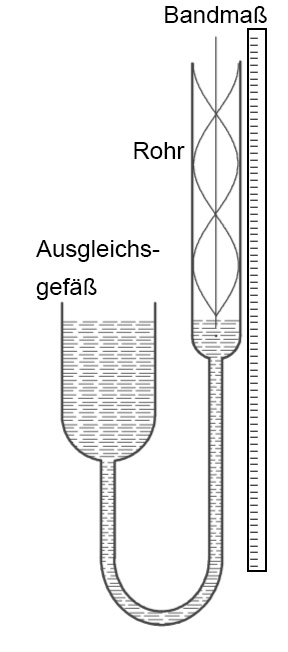
\includegraphics[scale=0.5]{Abb1}
	\caption{Aufbau zum ersten Versuchsteil: Ein quinckeschen Rohr.}
\end{figure}
Für den ersten Versuchsteil wurde ein Quinckesches Resonanzrohr verwendet (Siehe Abbildung 1). 

% describe set up
% insert pic name, designation, toc caption, caption, label
%\halftime{5}{5}{TEXT}{\fbox{\includegraphics[width=0.5\textwidth]{NAME}}
%   \renewcommand\thefigure{BX}
%\caption[XXXX]{XXXX \cite{Anleitung}}
%\label{Pic:X}}

\subsection{Durchführung}
Die Frequenzgenerator und der Oszillator wurden angeschaltet. Es wurde dann ein Frequenz zwischen 2 kHz und 7 kHz ausgewählt. Die Wasserhöhe in dem Rohr wurde dann verkleinert, indem man der Ausgleichsgefäß senkt. Als eine maximale Amplitude in dem Oszilloskop beobachtet wurde, wurde die Höhe des Wasserspiegels in dem Rohr mit einem Maßband gemessen. Dies wurde auch gemessen, als ein Minimum beobachtet wurde. Für jede Frequenz wurden die Wasserhöhe für 8-10 Maximum und Minimum gemessen. Es wurden drei Unterschiedliche Frequenzen untersucht. 


\subsection{Auswertung und Fehleranalyse}

XXXX

\section{Diskussion der Ergebnisse}

XXXX

\pagebreak

\section{2. Versuchsteil: Bestimmung der Ultraschallgeschwindigkeit durch die Messung der Wellenlänge.}
\subsection{Theorie}
\subsection{Aufbau}
\begin{figure}
	\centering
	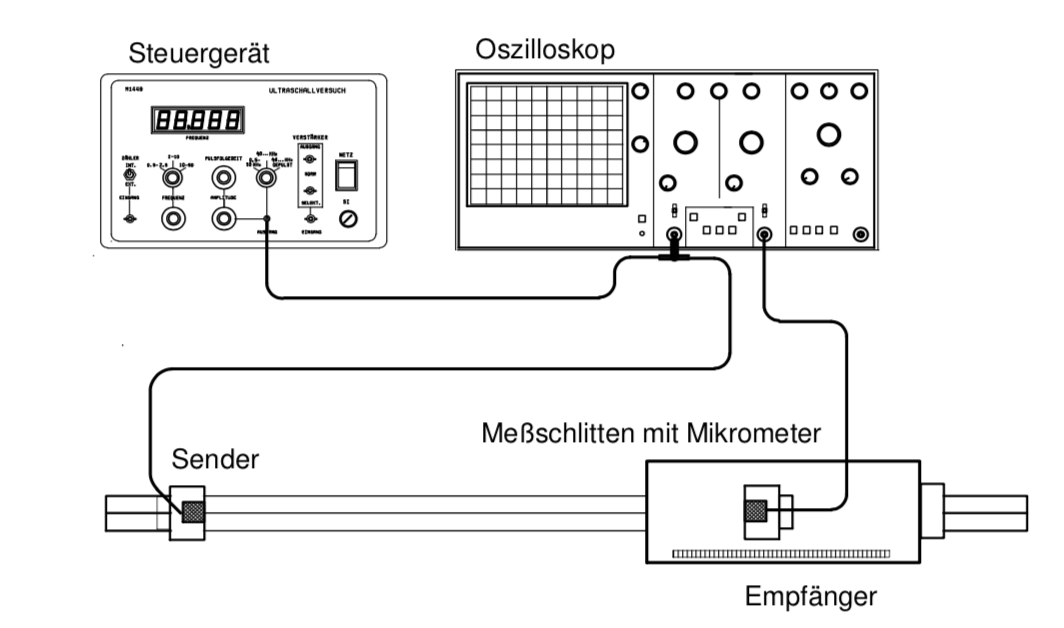
\includegraphics[scale=0.5]{Abb2}
	\caption{Aufbau zum zweiten Versuchsteil}
\end{figure}

Für diesen Versuchsteil wurden ein Ultraschallsender und -empfänger, ein Oszilloskop, ein Signalgenerator und ein Mikrometerschraube (Siehe Abbildung 2). 

\subsection{Durchführung}
Der Sender und der Empfänger (mit dem Mikrometerschraube) wurden auf beiden Seiten der Bank fixiert. Der Oszilloskop wurde angeschaltet und justiert, sodass beide Signale im Bildschirm zu sehen waren. Der Empfänger wurde dann mit dem Mikrometerschraube verschoben, sodass die zwei angezeigten Signalen in Deckung waren. Sein Position relativ zum Mikrometerschraube wurde dann aufgenommen. Der Empfänger wurde dann wiederum mit dem Mikrometerschraube verschoben, bis die zwei Signalen wieder in Deckung waren. Seine Position wurde dann aufgenommen. Die Positionen wurde 10-mal für jedes mal, dass die zwei Signalen in Deckung waren, gemessen. Dieser Prozess wurde für vier verschiedene Startpositionen des Empfängers wiederholt. 



\subsection{Auswertung und Fehleranalyse}
\subsection{Diskussion der Ergebnisse}

\section{3. Versuchsteil: Bestimmung der Ultraschallgeschwindigkeit durch die Messung der Laufzeit}

\subsection{Theorie}
\subsection{Aufbau}
\begin{figure}
	\centering
	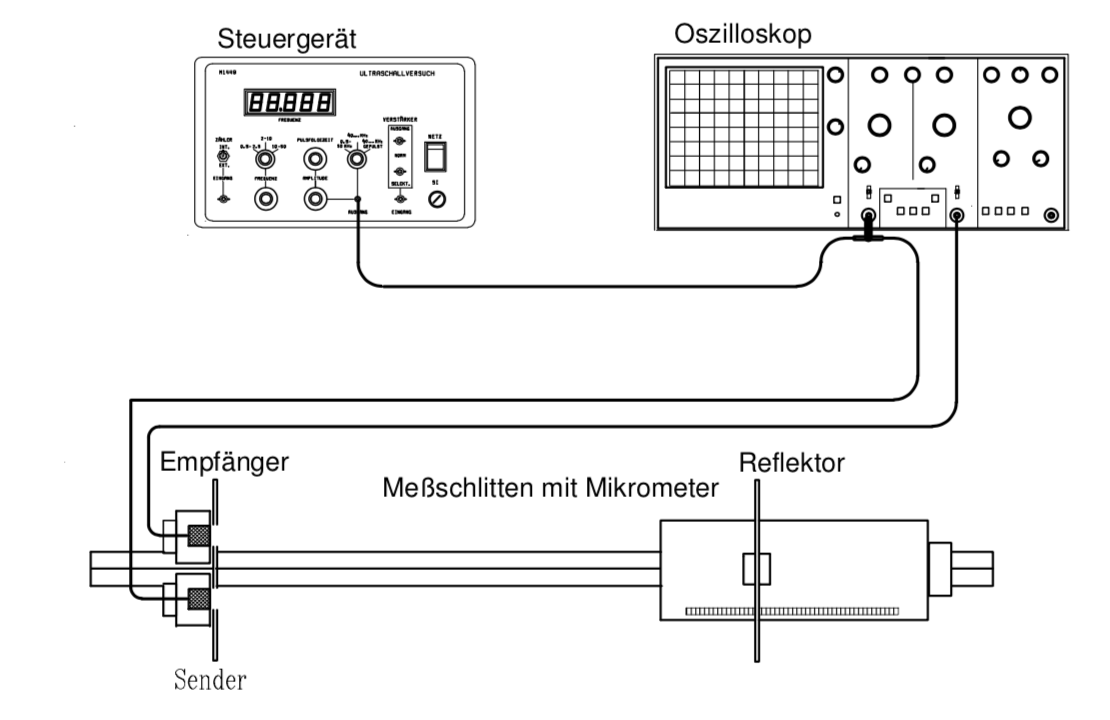
\includegraphics[scale=0.5]{Abb3}
	\caption{Aufbau zum dritten Versuchsteil}
\end{figure}
Für diesem Versuchsteil wurden dieselben Apparate wie in dem zweiten Teil und ein Reflektor benutzt (Siehe Abbildung 3). 

\subsection{Durchführung}
Zu diesem Versuchsteil wurde der Empfänger und der Sender auf derselben Seite der Bank fixiert. Auf der anderen Seite wurde ein Reflektor installiert. Es wurde die Betriebsart 3 des Frequenzgenerators ausgewählt. Der Oszilloskop und Frequenzgenerator wurden angeschaltet und justiert, sodass zwei Pulse im Bildschirm des Oszilloskops zu sehen waren. Der Abstand zwischen dem Empfänger-Sender Komplex und dem Reflektor wurde mit einem Maßband gemessen. Der Zeitdauer zwischen dem ausgesandten Puls und empfangenen Puls wurde direkt mithilfe der Skala auf dem Oszilloskop gemessen. 

\section{Anhang: Tabellen und Diagramme}

\begin{table}[h]
\centering
\caption{XXXX} \vspace{11pt}
$\begin{array}{l}
\textrm{Unsicherheiten:}\\
\textrm{XXXX: } \pm XX \textrm{XX}\\
\end{array}$
\begin{tabular}{ccc}
\toprule
\textrm{XXXX}/\textrm{XX} & \textrm{XXXX}/\textrm{XX} & \textrm{XXXX}/\textrm{XX} \\
\midrule 
2 & 0.26 & 0.23\\
\hline
4 & 0.33 & 0.25\\
\hline 
5 & & 0.3\\
\hline 
6 & 1.25 & 0.83\\
\hline 
8 & 3.9 & 0.83\\ 
\hline
9 & 4.75 & 4.6\\ 
\hline
10 & 4.7 &\\ 
\bottomrule
\end{tabular}
\phantom{$\begin{array}{l}
\textrm{Unsicherheiten:}\\
\textrm{XXXX: } \pm XX \textrm{XX}\\
\end{array}$}
\label{Tab:X}
\end{table}

%\begin{figure}[p]
%\centering
%\fbox{\includegraphics[width=0.8\textwidth]{NAME}}
%\renewcommand\thefigure{BX}
%\caption[XXXX]{XXXX}
%\label{Abb:X}
%\end{figure}

\begin{thebibliography}{9}
\bibitem{Uncertainties}''Correlations between variables are automatically handled, which sets this module apart from many existing error propagation codes.'' - https://pythonhosted.org/uncertainties/
\bibitem{Anleitung} Physikalisches Institut der Albert-Ludwigs-Universität Freiburg (Hrsg.) (08/2018): Versuchsanleitungen zum Physiklabor für Anfänger*innen, Teil 1, Ferienpraktikum im Sommersemester 2018.
\end{thebibliography}

\end{document}